\section{Week 3 - Object detection}
Learn how to apply your knowledge of CNNs to one of the toughest but hottest field of computer vision: Object detection.
\subsection{Detection algorithms}
\subsubsection{Object Localization}
Defining the target label y

\begin{enumerate}
    \item pedestrian
    \item car
    \item motorsycle
    \item background
\end{enumerate}
Need to output the bounding box for the detected object (center point of the object $b_x$, $b_y$, height $b_h$, width $b_w$) and a class label (1-4)

y is a vector that starts with $p_c$ whether there is an object in the image or not. It's a supervisod learning algorithm, your labeled data should contain also the boxes.

\begin{equation*}
    \mathcal{L}(\hat{y}, y) = \left\{
                \begin{array}{ll}
                  (\hat{y}_1-y_1)^2 + (\hat{y}_2-y_2)^2 + . . . + (\hat{y}_8-y_8)^2 if y_1= 1\\
                  (\hat{y}_1-y_1)^2 if y_1= 0
                \end{array}
              \right.
\end{equation*}

\subsubsection{Landmark Detection}
Example detect emotion from detecting landmarks (e.g. eyes, nose) in a person's face. Detecting pose of a person, determine the key landmarks: arm, chase, etc.

\subsubsection{Object Detection}
Car detection example: crop pictures of cars to build a labeled dataset that you can train with a ConvNet to detect this object (i.e. car).
With \textbf{Sliding Window} algorithm, you can take a region and move it on your original picture then feed this region to your ConvNet to detect a car there.

A disadvantage of the sliding window is it's high computation cost as you try different sizes of region and having to move these regions across the picture.

\subsubsection{Convolutional Implementation of Sliding Windows}
Bsically, this algorithm turns the fully connected layers into convolution layers then pass the whole image and result is a cell of every possible region you would have cropped with the previous algorithm.

The convolution implementation is it combines all four into one form of computation and shares a lot of the computation in the regions of image that are common, instead of instead of forcing you to run four propagation on four subsets of the input image independently.

One problem of this algorithm is that the resulting bounding boxes are not accurate.

\subsubsection{Bounding Box Predictions}
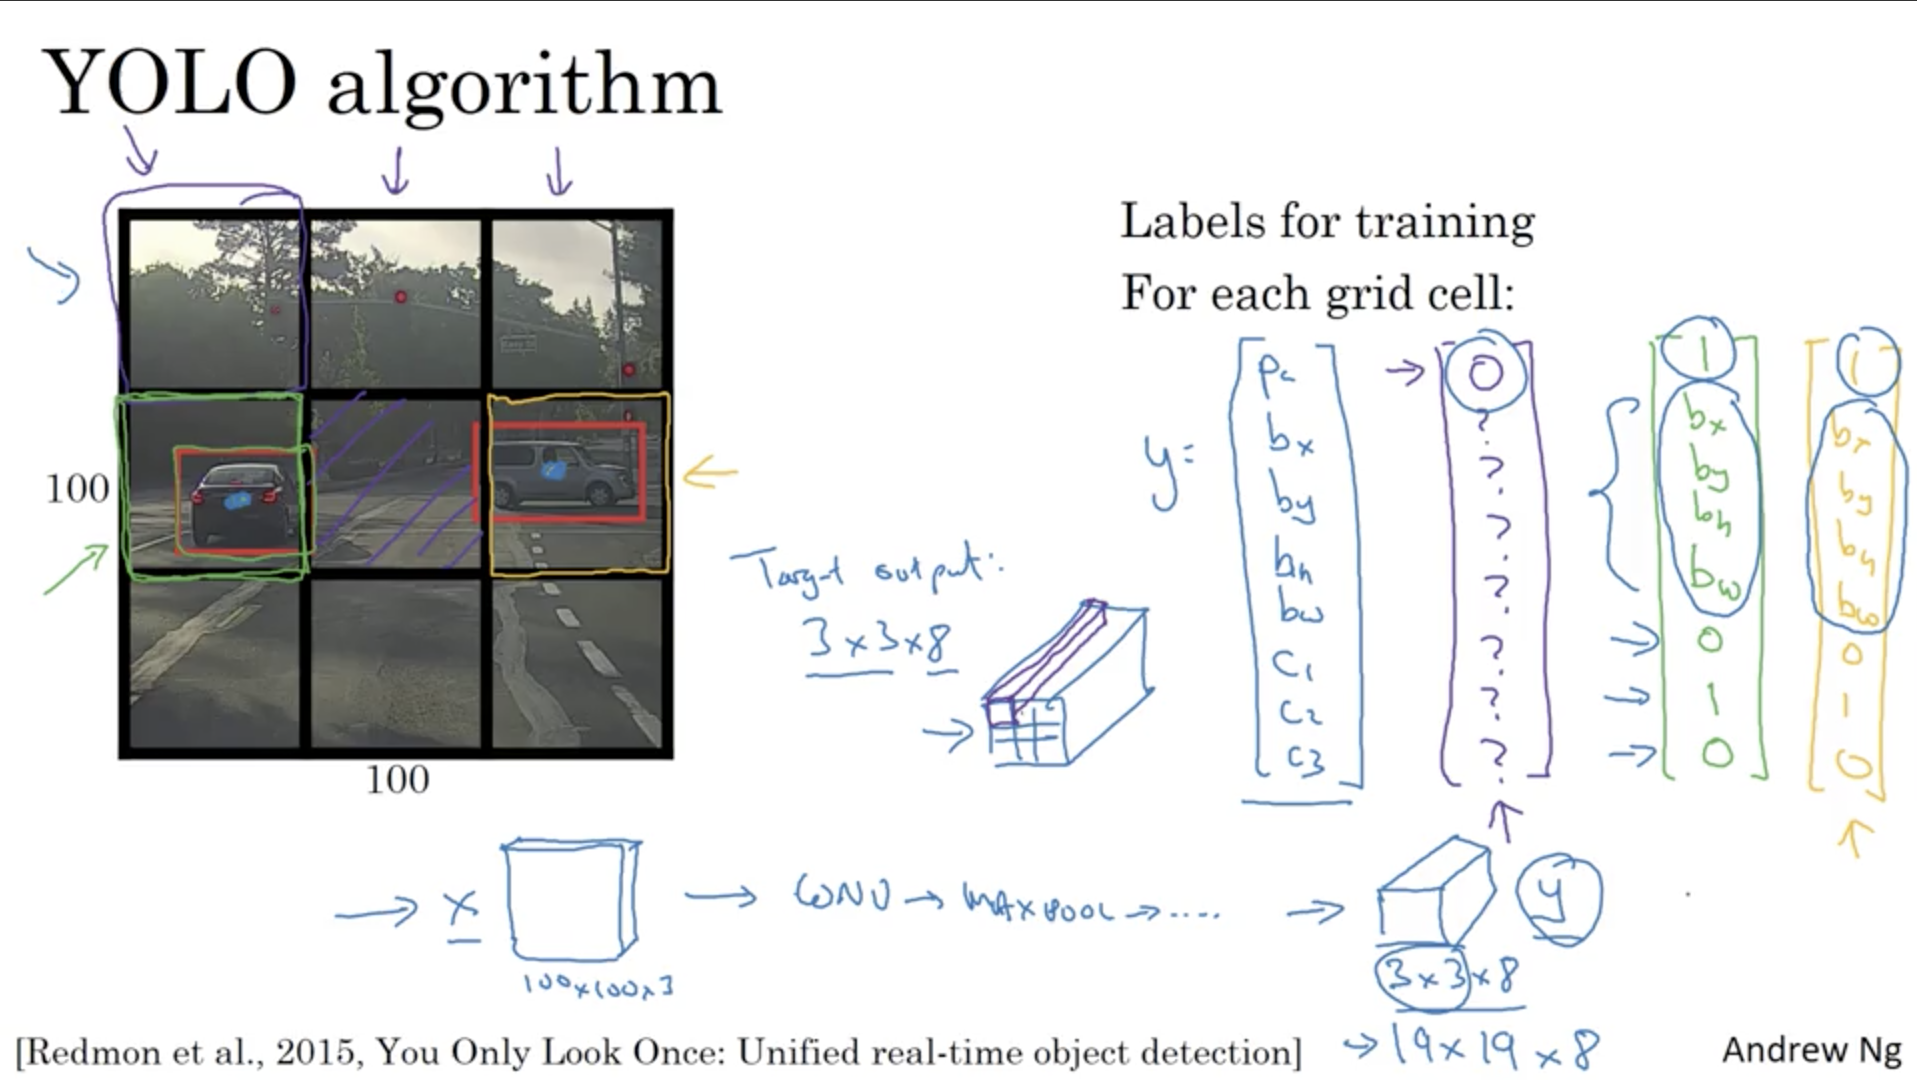
\includegraphics[scale=0.35]{Bounding_Box_Predictions_YOLO_Conv_Impl}

\subsubsection{Intersection Over Union}
Function for evaluating a detection algorithm. IOU computes the intersection of the bounding boxes divided by the size of the union of both boxes (the real one, and the predicted one).
\begin{equation*}
    IOU = \frac{\text{size of intersection}}{\text{size of union}}
\end{equation*}
Correct if $IOU \ge 0.5$

\subsubsection{Non-max Suppression}
It's way to make sure an object is detected by your algorithm only once. This by taking the max of the $p_c$ probabilities of the bounding boxes.

Algorithm:
\begin{itemize}
    \item divide the input picutre in a grid of 19x19 cells
    \item the output will be 19x19x8, where each cell is 8 length vector (see above)
    \item discard all boxes with probablity $p_c \leq 0.6$
    \item while there are any remaining boxes:
    \begin{itemize}
        \item Pick the box with the largest $p_c$, output that as a prediction
        \item Discard any remaining box with $IOU \ge 0.5$ with the box output in the previous step.
    \end{itemize}
\end{itemize}

\subsubsection{Anchor Boxes}
One of the problem object detection algorithm is that if a pedestrain and a car has same center, then the algorithm may pick one object over the other and not both. To avoid this use anchors of different shapes.

\begin{itemize}
    \item \textbf{Previously:} Each object in training image is assigned to grid cell that contains that object’s midpoint.
    \item \textbf{With two anchor boxes:} Each object in training image is assigned to grid cell that contains object’s midpoint and anchor box for the grid cell with highest IoU.
\end{itemize}
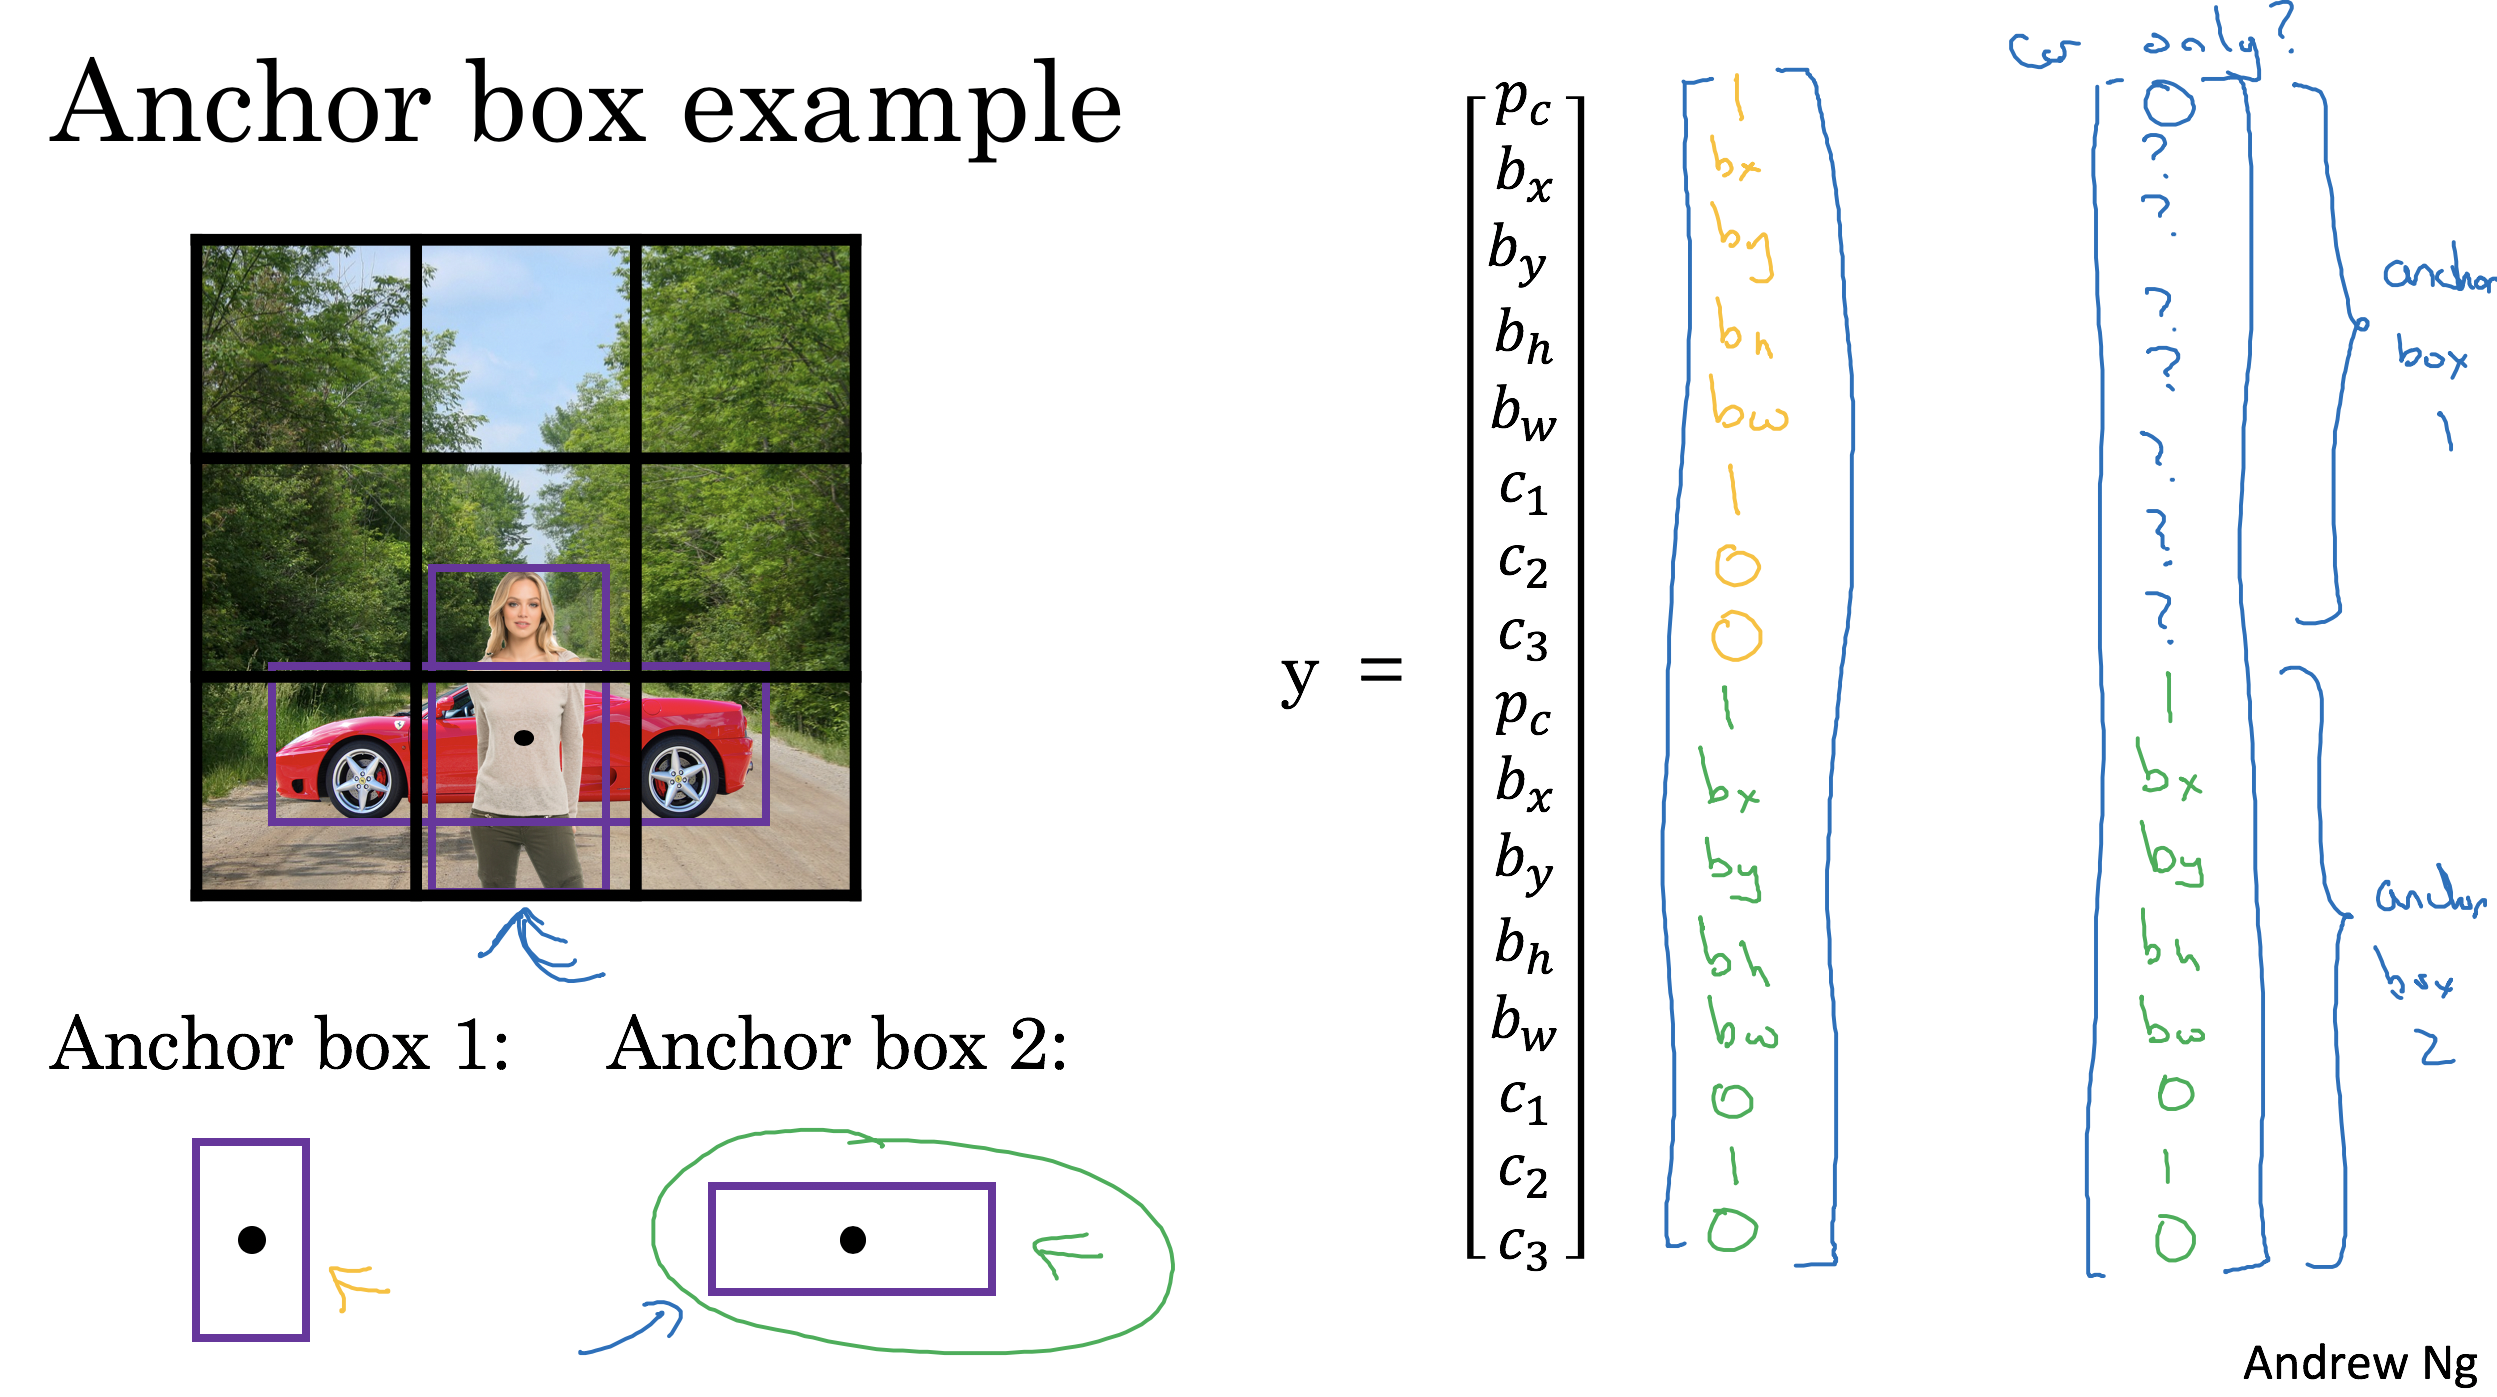
\includegraphics[scale=0.35]{Anchor_Boxes}
This algorithm allows your learning algorithm to specialize better, in detecting fat, skinny objects.

\subsubsection{YOLO Algorithm}
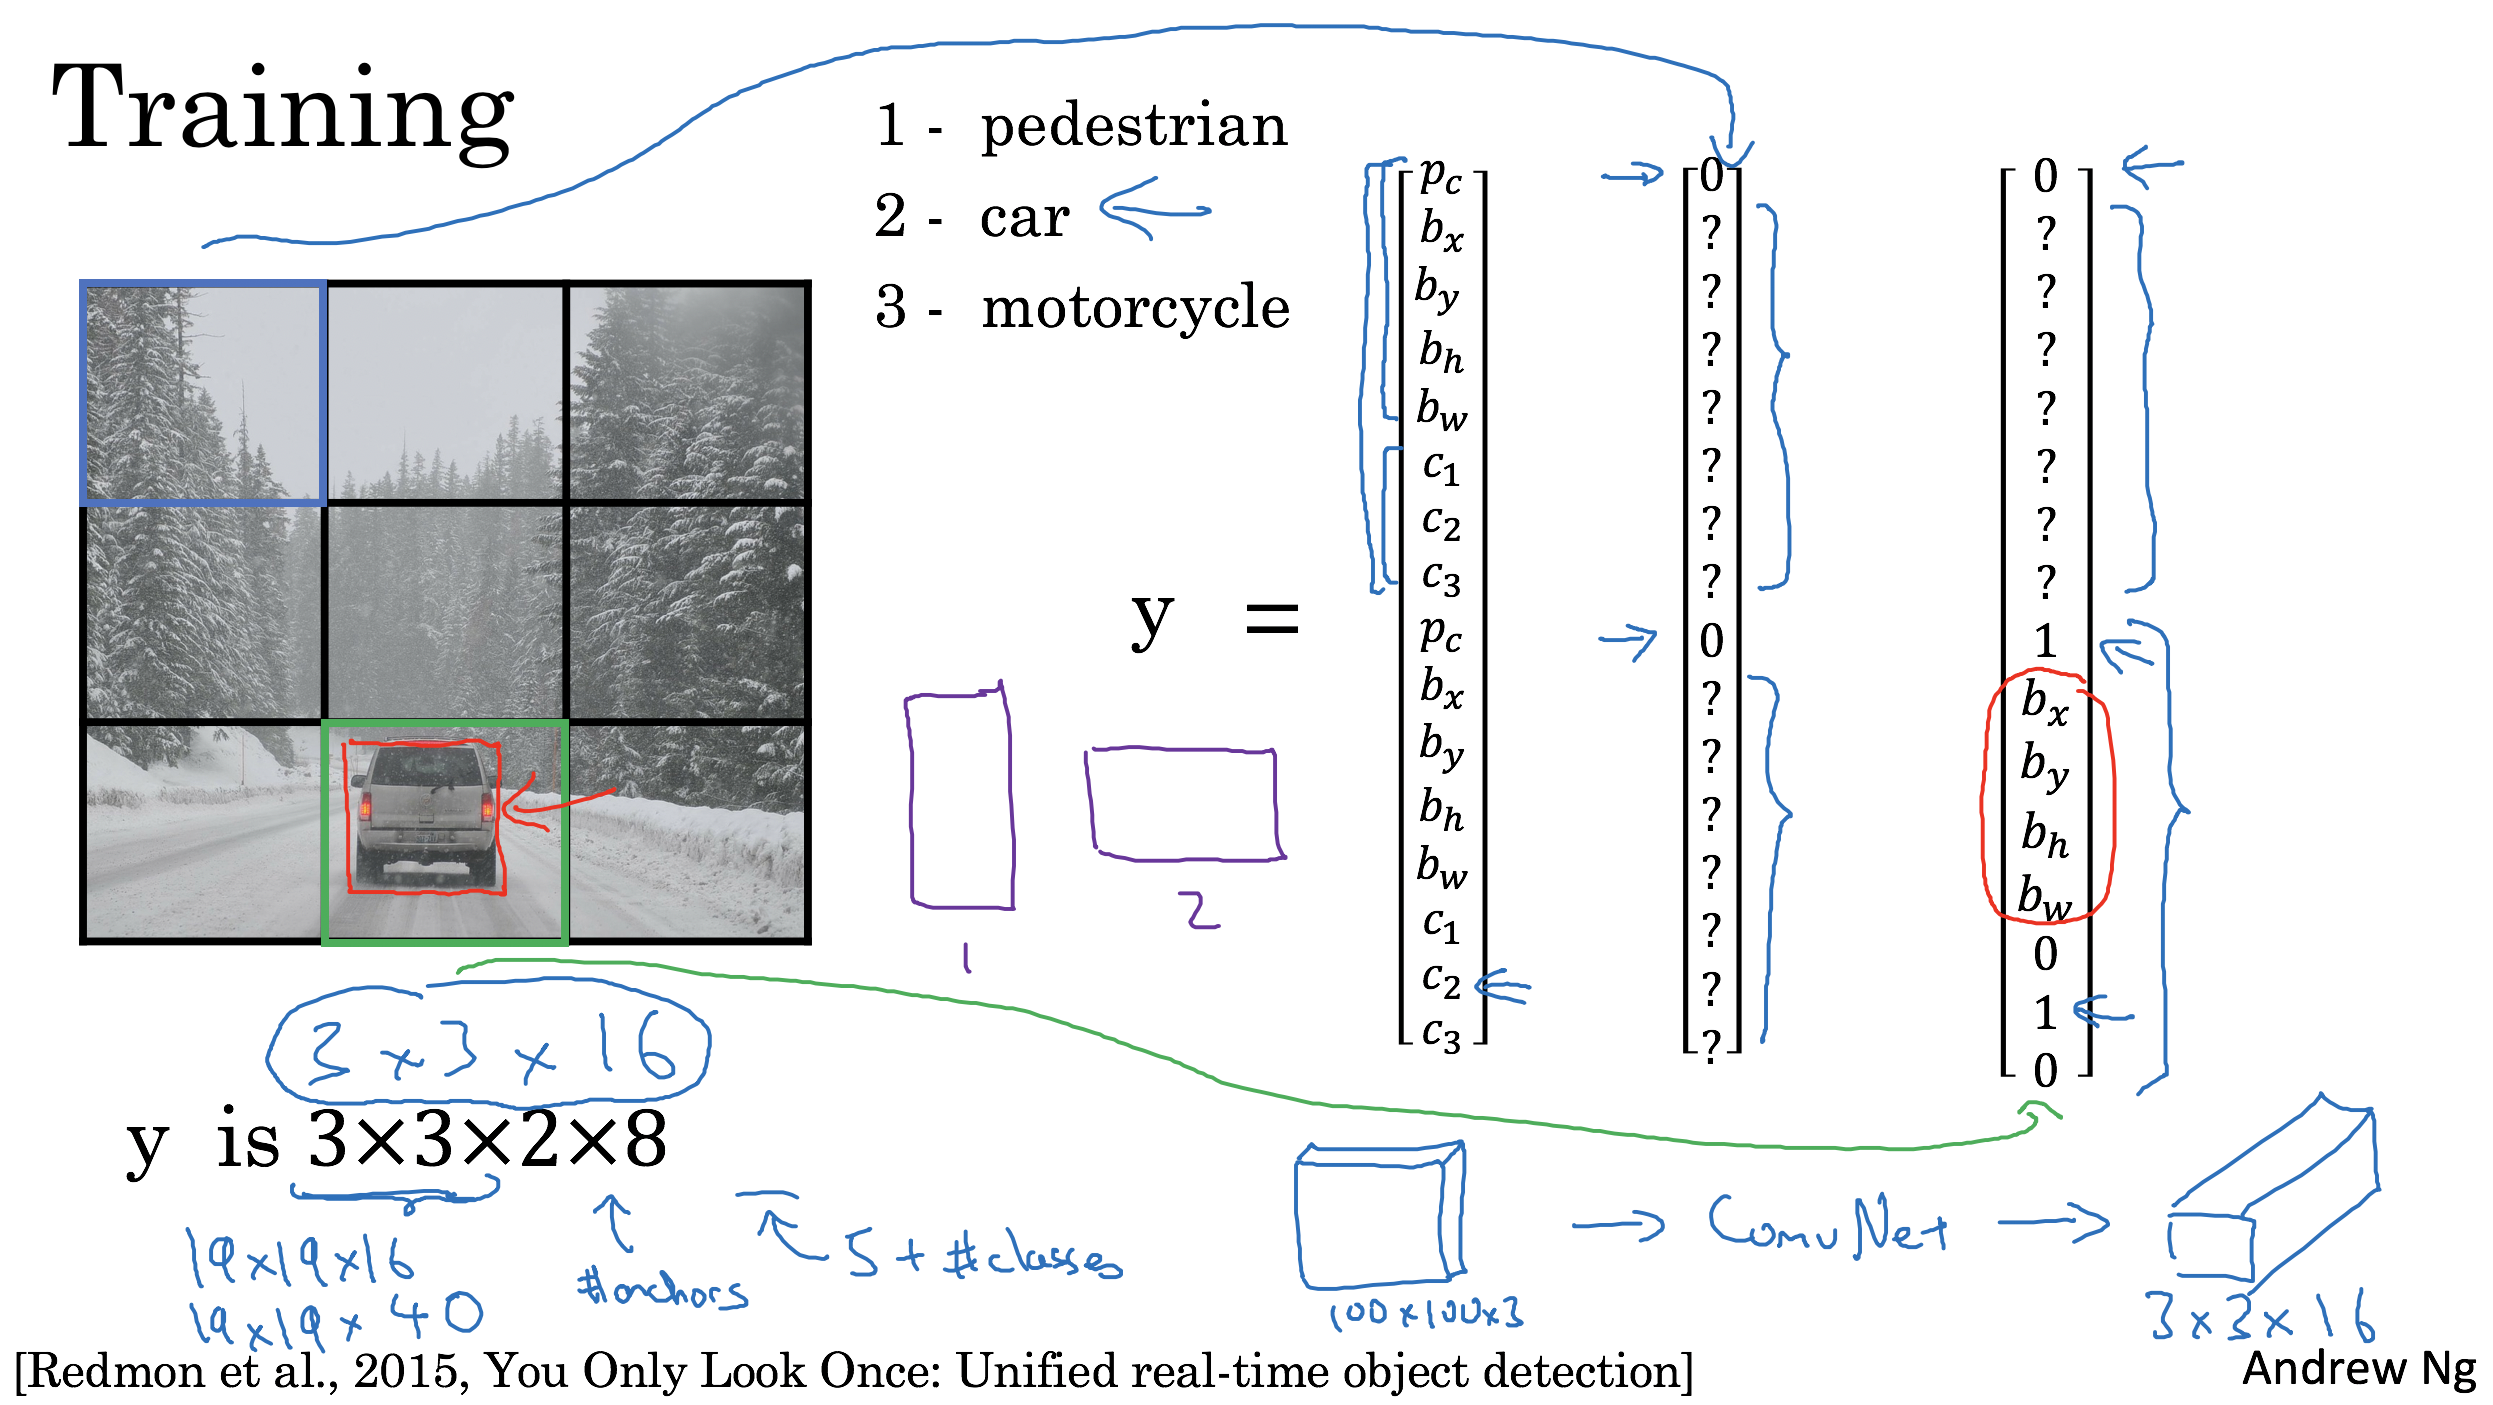
\includegraphics[scale=0.35]{YOLO_algorithm_training}

Outputting the non-max supressed outputs
\begin{itemize}
    \item For each grid call, get 2 predicted bounding boxes. 
    \item Get rid of low probability predictions.
    \item For each class (pedestrian, car, motorcycle) use non-max suppression to generate final predictions.
\end{itemize}

\subsubsection{(Optional) Region Proposals}
Run a segmentation algorithm to detect what could be an object, blobs (e.g. 2000), then run ConvNet on those regions.

The based Rregion CNN is quite slow, alternative Faster algorithms
\begin{itemize}
    \item \textbf{R-CNN:} Propose regions. Classify proposed regions one at a time. Output label + bounding box.
    \item \textbf{Fast R-CNN:} Propose regions. Use convolution implementation of sliding windows to classify all the proposed regions.
    \item \textbf{Faster R-CNN:} Use convolutional network to propose regions.
\end{itemize}

\subsection{Practice questions}
\subsubsection{QUIZ - Detection algorithms}
\textbf{1.} You are building a 3-class object classification and localization algorithm. The classes are: pedestrian (c=1), car (c=2), motorcycle (c=3). What would be the label for the following image? Recall $y = [p_c, b_x, b_y, b_h, b_w, c_1, c_2, c_3]$.
\begin{itemize}
    \item $y=[1,0.3,0.7,0.3,0.3,0,1,0]$ (X)
    \item $y=[1,0.7,0.5,0.3,0.3,0,1,0]$
    \item $y=[1,0.3,0.7,0.5,0.5,0,1,0]$
    \item $y=[1,0.3,0.7,0.5,0.5,1,0,0]$
    \item $y=[0,0.2,0.4,0.5,0.5,0,1,0]$
\end{itemize}
\textbf{2.} Continuing from the previous problem, what should y be for the image below? Remember that “?” means “don’t care”, which means that the neural network loss function won’t care what the neural network gives for that component of the output. As before, $y = [p_c, b_x, b_y, b_h, b_w, c_1, c_2, c_3]$.
\begin{itemize}
    \item $y=[1,?,?,?,?,0,0,0]$
    \item $y = [0, ?, ?, ?, ?, 0, 0, 0]$
    \item $y = [1, ?, ?, ?, ?, ?, ?, ?]$
    \item $y = [?, ?, ?, ?, ?, ?, ?, ?]$
    \item $y = [0, ?, ?, ?, ?, ?, ?, ?]$ (X)
\end{itemize}
\textbf{3.} You are working on a factory automation task. Your system will see a can of soft-drink coming down a conveyor belt, and you want it to take a picture and decide whether (i) there is a soft-drink can in the image, and if so (ii) its bounding box. Since the soft-drink can is round, the bounding box is always square, and the soft drink can always appears as the same size in the image. There is at most one soft drink can in each image. Here’re some typical images in your training set:

What is the most appropriate set of output units for your neural network?
\begin{itemize}
    \item Logistic unit (for classifying if there is a soft-drink can in the image)
    \item Logistic unit, $b_x$ and $b_y$
    \item Logistic unit, $b_x, b_y, b_h$ (since $b_w = b_h$) (X 1)
    \item Logistic unit, $b_x, b_y, b_h, b_w$ (X 2)
\end{itemize}
\textbf{4.} If you build a neural network that inputs a picture of a person’s face and outputs N landmarks on the face (assume the input image always contains exactly one face), how many output units will the network have?
\begin{itemize}
    \item N
    \item 2N (X)
    \item 3N
    \item $N^2$
\end{itemize}
\textbf{5.} When training one of the object detection systems described in lecture, you need a training set that contains many pictures of the object(s) you wish to detect. However, bounding boxes do not need to be provided in the training set, since the algorithm can learn to detect the objects by itself.
\begin{itemize}
    \item True (X 1)
    \item False (X 2)
\end{itemize}
\textbf{6.} Suppose you are applying a sliding windows classifier (non-convolutional implementation). Increasing the stride would tend to increase accuracy, but decrease computational cost.
\begin{itemize}
    \item True
    \item False (X)
\end{itemize}
\textbf{7.} In the YOLO algorithm, at training time, only one cell ---the one containing the center/midpoint of an object--- is responsible for detecting this object.
\begin{itemize}
    \item True (X)
    \item False
\end{itemize}
\textbf{8.} What is the IoU between these two boxes? The upper-left box is 2x2, and the lower-right box is 2x3. The overlapping region is 1x1.
\begin{itemize}
    \item 1/6
    \item 1/9 (X 2) $\frac{1}{1-1+2*2+2*3}$
    \item 1/10 (X 1)
    \item None of the above
\end{itemize}
\textbf{9.} Suppose you run non-max suppression on the predicted boxes above. The parameters you use for non-max suppression are that boxes with probability $\leq$ 0.4 are discarded, and the IoU threshold for deciding if two boxes overlap is 0.5. How many boxes will remain after non-max suppression?
\begin{itemize}
    \item 3
    \item 4 (X 1)
    \item 5 (X 2)
    \item 6
    \item 7
\end{itemize}
\textbf{10.} Suppose you are using YOLO on a 19x19 grid, on a detection problem with 20 classes, and with 5 anchor boxes. During training, for each image you will need to construct an output volume yy as the target value for the neural network; this corresponds to the last layer of the neural network. (yy may include some “?”, or “don’t cares”). What is the dimension of this output volume?
\begin{itemize}
    \item 19x19x(5x25) (X 2)
    \item 19x19x(20x25)
    \item 19x19x(5x20) (X 1)
    \item 19x19x(25x20)
\end{itemize}